In this section we will provide the methods of solar cell characterisation and the quantities which are connected to it.
 
\subsection{Solar Cell Operation}

For a solar cell to generate current, the following main processes must be present. First one is the possibility to absorb photons from incident light so we can generate carriers. We must remember that minority carriers are only stable for a minority carrier lifetime before recombination. Therefore, before this time, we need to collect those carriers to spatially disallow carriers to recombine. Ideally, if we create pair in the n region, the electric field sweeps the minority carrier through the junction to the place where it becomes majority carrier. In a short circuit situation, two carriers ideally meet together after flowing through the external circuit. 

The fact that the carriers must "live" through the distance needed to separate them is described by collection probability, which depends on the diffusion length and surface properties. 

The number of carriers collected in the solar cell compared to the number of incident photons describes the more macroscopic ability of the device. It is called a \textbf{quantum efficiency} $Q.E=\frac{number of carriers collected}{number of incident photons}$. It is strictly dependent also on the absorption so directly on the wavelength of incident photons. 

\begin{figure}
\centering
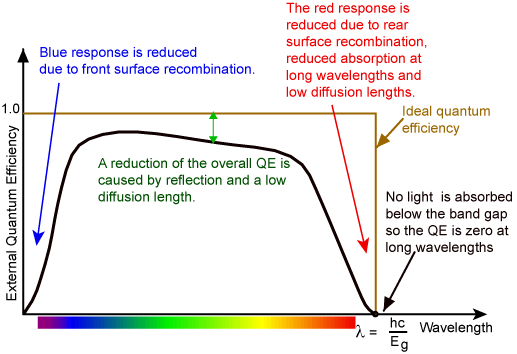
\includegraphics[width =0.6\textwidth]{ch2/QE}
\caption{Quantum efficiency of an ideal silicon solar cell \cite{pv}}
\end{figure}

It is also possible to describe an external QE, which also includes some optical effect such as reflection. 

\subsection{Solar Cell Parameters}
Here, we will state the most important parameters for solar cell characterisation, we will simply tell what do they stand for and how to measure them. 

\subsubsection{Short-Circuit Current}
$I_{sc}$ is the current that flows through the device providing that the voltage is zero across it(especially when we have short circuit). It comes directly from the generated carriers due to photogeneration and is connected to how well the structure can collect them or how strong the recombination processes are. It depends on:

\begin{itemize}
\item incident photons number(linear dependence on the incident power)
\item solar cell area
\item light spectrum
\item optical losses(f.e. absorption, reflection etc.)
\item real collection efficiency(its' probability)
\end{itemize}

We can clearly see, that this parameter allows us to differentiate between solar cells when comparing the ability to store generated carriers.(Remember, short-circuit current is not always the light generated current due to possible high series resistance).

\subsubsection{Open-Circuit Voltage}

$V_{oc}$ is the voltage that is maximally available when using the solar cell. For that voltage, the current through the circuit needs to be zero. It states the forward bias that we need to put to compensate the light generated current. $V_{oc}$ is logarithmically dependent on the incident photon power and it decreases linearly with temperature. 

\subsubsection{Fill Factor}

\subsubsection{PCE}

\subsection{Effective resistance}

\subsection{Shockley-Queisser limit}